\newpage
\section{Decision Trees}\label{s:decision-trees}

Decision trees are tree-like structures in which each internal node represents a ``test" on an attribute, each branch represents the outcome of the specific test, and each leaf node represents a class label (decision taken after computing all attributes).
More specifically, decision trees depict models of decisions and their possible results.
They are also a simple way to display an algorithm that only contains conditional control statements.
Starting from the root node and following the paths to leaves, each path represents classification rules.

For instance, the attribute ``Gender" would have two edges leaving it, one for ``Male" and
one for ``Female".
Each edge could point to a new attribute (for example ``Age Groups"), and so on.
The leaves of the tree contain the expected class value for transactions matching the path from the root to that leaf.
Given a decision tree, one can predict the class of a new transaction just by following the ``correct" path, which will result in a class label.
He/She can predict the class of a transaction by viewing only the non-class attributes (i.e. the ``constructed" decision tree).

For instance, two friends wish to decide if they will go to play tennis outside, depending the weather conditions.
They also remember the previous days that some weather conditions did not allow them to play.
Thus, they decide to create a decision tree to assist them.
First they define the class attribute to be ``Play Tennis", and three more attributes that will help them decide: ``Outlook" (``Sunny", ``Overcast", ``Rainy"), ``Windy" (``High", ``Low") and ``Humidity" (``High", ``Low").
Then they construct a decision tree like figure \ref{f:outlook} that corresponds to the data that the have collect from the past days.

\begin{figure}[th]
  \centering
  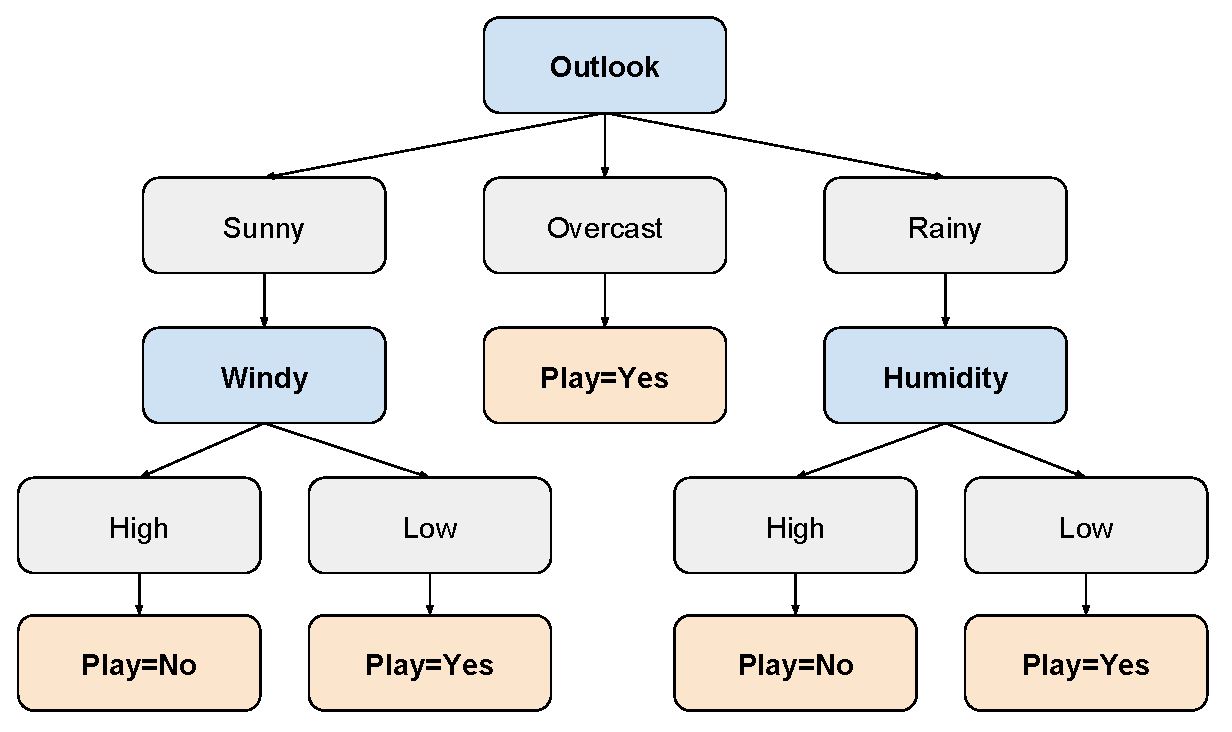
\includegraphics[width=0.8\linewidth]{figures/outlook.pdf}
  \caption{Play-Tennis decision tree example}\label{f:outlook}
\end{figure}

From figure \ref{f:outlook}, the two friends are able to extract a set of rules, listed in Code \ref{sc:outlook-rules}, that will help them decide if they should go play tennis given the weather conditions.

{
\begin{minted}[xleftmargin=21pt, framesep=3mm, frame=single, linenos, tabsize=2, breaklines, breaksymbolleft=, fontsize=\footnotesize]{bash}
IF (Outlook = Sunny) AND (Windy = Low) THEN Play=Yes

IF (Outlook = Sunny) AND (Windy = High) THEN Play=No

IF (Outlook = Overcast) THEN Play=Yes

IF (Outlook = Rainy) AND (Humidity = High) THEN Play=No

IF (Outlook = Rainy) AND (Humidity = Low) THEN Play=Yes
\end{minted}
\captionof{lstlisting}{Rules for decision tree from figure \ref{f:outlook}}
\label{sc:outlook-rules}
}

Of course, remembering the weather conditions of more days in the past and if they had played tennis those days -- having an extended dataset -- could probably result to more specific rules.
Decision tree rules, help covering all possible future decisions\hyp transactions and can be used to classify them.
There are many useful examples and it has become evident why this type of learning has become so popular.
The algorithms according to which those tress are generated vary and lead to possible different trees.

One famous algorithm for decision tree construction is ID3 (Iterative Dichotomiser 3).
ID3 is the precursor to the C4.5 algorithm, and is typically used in the machine learning and natural language processing domains.
Both algorithms build decision trees from a set of training data, using the concept of information entropy, however, C4.5 results in better classification utilizing a more efficient splitting criterion.




\subsection{Textbook ID3}\label{s:id3}

The ID3 algorithm was first introduced in \cite{quinlan1986induction} and assumes that each attribute is categorical, such as the aforementioned attribute ``Age Groups" which is separated in four disjoint categories; ``Infant", ``Adolescent", ``Child" and ``Adult".

ID3 algorithm constructs the classification tree top-down in a recursive fashion.
The idea is to find the \textit{best} attribute that classifies the transactions.
At start, the algorithm searches and chooses the best attribute for the root node, and consecutively the remaining transactions are partitioned by it.
On each partition, ID3 is then recursively called.

The \textit{best} attribute is defined as the attribute that has the smallest entropy -- or in other words, the best information gain.
Let $T$ be a set of transactions, $C$ the class attribute and $A$ some non-class attribute.
On each iteration, ID3 iterates through every unused attribute $A$ of the dataset and calculates the entropy $H_C(T)$ (equation \ref{eq:entropy} and algorithm \ref{a:id3-entropy-simple}) for every subset $T$ that results from splitting the dataset on attribute $A$.

\import{./}{algorithms/entropy_textbook.tex}

\begin{equation}\label{eq:entropy}
  H_C(T) = \sum_{i=1}^{l} - \frac{\mid T(c_i) \mid}{\mid T \mid} log{\frac{\mid T(c_i) \mid}{\mid T \mid}}
\end{equation}

The idea is to identify the class of a transaction $t$, given that the value of $A$ has been obtained.
Let $A$ obtain values $a_1, \dots, a_m$ and let $T(a_j)$ be the transactions obtaining value $a_j$ for $A$.
Then, the conditional information of $T$ given $A$, is given from equation \ref{eq:TgivenA}.

\import{./}{algorithms/gain_textbook.tex}

\import{./}{algorithms/best_textbook.tex}

\begin{equation}\label{eq:TgivenA}
  H_C(T \mid A) = \sum_{j=1}^{m} - \frac{\mid T(a_j) \mid}{\mid T \mid} H_C(T(a_j))
\end{equation}

\begin{equation}\label{eq:gain}
  Gain(A) = H_C(T) - H_C(T \mid A)
\end{equation}


Finally, the set $T$ is then split by the selected attribute $A$ (best-attribute algorithm \ref{a:id3-best-simple}) that has the maximum gain (equation \ref{eq:gain} and algorithm \ref{a:id3-gain-simple}) -- or equivalently minimum $H_C(T \mid A)$ -- to produce subsets of the data.
The algorithm continues to recurse on each subset, considering only attributes never selected before.

The \f{AllExamplesSame} (see algorithm \ref{a:id3-same-simple}) procedure is used to determine if all transactions are of the same class, by checking the value of $classAttribute$ for each transaction.
It returns $true$ if they are, $false$ otherwise.

\import{./}{algorithms/allsame_textbook.tex}

The \f{MostCommonLabel} (algorithm \ref{a:id3-most-common-label-simple}) procedure returns the class label that is most common in all available transactions.

\import{./}{algorithms/most_common_label_textbook.tex}

The recursive \f{ID3} algorithm (see algorithm \ref{a:id3-simple} shown below) has the following structure with three halting conditions.
\begin{enumerate}
  \item If the set of remaining attributes is empty, then the algorithm returns the label that is most common in all transactions as a leaf (lines 2-3).
  \item If all transactions are of the same class, then the algorithm returns this class as a leaf (lines 4-5).
  \item If none of the above conditions hold, then the algorithm finds the best splitting attribute (using algorithm \ref{a:id3-best-simple}) and makes a branch for every possible value of that attribute (lines 7-19).
\end{enumerate}

\import{./}{algorithms/id3_textbook.tex}



\subsection{Privacy Preserving ID3}\label{s:pp-id3}

In the previous subsection we described the ID3 algorithm which operates on public data.
We should now describe the privacy\hyp preserving version of the same algorithm, where all the transactions (\textit{examples}) from which the algorithm builds the tree are private data.

First of all, a key difference from the textbook algorithm is the lack of ability to maintain subsets of the transactions based on private conditions.
In particular, as you can see in line 11 of algorithm \ref{a:id3-simple}, we wish to keep a subset of all $examples$ that have a certain value in the $bestAttribute$
 column.

As we cannot have conditional statements on private data, the only thing we can do is to apply the oblivious selection technique described in section \ref{s:secrec}.
Thus, we are not able to keep only the subset of rows that satisfy our condition.
A solution to this problem is to define $subset$ as a copy of the $examples$ array.
We keep a vector $eq$ (see line 17 of algoritm \ref{a:id3-pp}) of equal length with $examples$.
The value of $eq[i]$ is $\enc{1}$ if $examples[bestAttribute]$ is equal to $v_i$, or $\enc{0}$ otherwise.
Since the values of $eq$ are encrypted, we perform a vector multiplication between $eq$ and $examples$ so the result will be identical to $examples$ for ever row $i$ that the condition holds ($eq[i]$ is equal to $\enc{1}$), and $\enc{0}$ otherwise.
Then we add a dummy row $[\enc{-1}, \enc{-1}, \dots, \enc{-1}]$ (a row of all $\enc{-1}$, denoted as just $\enc{-1}$ for simplicity) to all rows that don't satisfy the condition (using multiplication with $\enc{1} - eq$).
The resulting array has all rows from $examples$ that satisfy the condition, and rows full of $\enc{-1}$ wherever the condition does not hold.

For that reason, all the algorithms listed below operate on these kinds of ``sets''.
In algorithm \ref{a:id3-count-positives-pp} we describe the \f{CountPositives} procedure which returns the (encrypted) number of rows that are not the dummy $[\enc{-1}, \enc{-1}, \dots, \enc{-1}]$ row.
The \f{CountPositives} procedure is equivalent to the call of $Length$ on sets with public data.


\import{./}{algorithms/count_positives.tex}

The \f{AllExamplesSame} procedure described in algorithm \ref{a:id3-same-pp} returns the same result as that in algorithm \ref{a:id3-same-simple}.
The way this is achieved is by counting the number of examples / transactions that are of class $c_i$, for each possible class $c_i$.
The private variable $res$ is initialized to $\enc{0}$, and gets increased if any of those counts is equal to the total number of examples, \textit{i.e.} all examples are of that class.
If $res$ is greater than $\enc{0}$ (equal to $\enc{1}$) then all the examples have the same class.

\import{./}{algorithms/allsame_pp.tex}

Similarly to the \f{AllExamplesSame} procedure, the \f{MostCommonLabel} procedure also maintains the transaction counts for each possible class $c_i$.
Using the technique described in algorithm \ref{a:max}, we obliviously keep the maximum count and the class label corresponding to that count, which is returned.

\import{./}{algorithms/most_common_label_pp.tex}

The \f{Best} procedure obliviously chooses the attribute that has the greatest information gain.
This attribute is considered to be the best to split the dataset on an will be included in an output tree node.
That is why this attribute can be handled as public data (note the usage of the \f{Declassify} operator in line 10) after it has been privately computed.


\import{./}{algorithms/best_pp.tex}

As in algorithms \ref{a:id3-entropy-simple} and \ref{a:id3-gain-simple}, procedures \f{Entropy} and \f{InformationGain} (algorithms \ref{a:id3-entropy-pp}, \ref{a:id3-gain-pp}) compute the entropy of a set of transactions, and an attribute's information gain respectively.
The key differences with the previously described textbook algorithms include the usage of \f{CountPositives} procedure instead of \f{Length}, due to the difference in the sets involved in the computation, and the modified $log_2$ function that handles zero input.
Also, note that the subsets (algorithm \ref{a:id3-gain-pp}, line 5) are also constructed with the technique described in the beginning of this section.


\import{./}{algorithms/entropy_pp.tex}
\import{./}{algorithms/gain_pp.tex}

The complete \f{ID3} procedure is described in algorithm \ref{a:id3-pp}.
In lines 6-11 of the algorithm we retrieve class label that is same to all examples ad return it.
In order to do that, we cannot just take a random's example value in the $classAttribute$ column.
We should make sure that this is not a dummy ($\enc{-1}$) example (line 8).
The rest of the algorithm is quite similar to the textbook one.
The differences mainly include the subsets handling. (creation, counting, etc.)


\import{./}{algorithms/id3_pp.tex}


\subsubsection{Privacy Assessment}\label{s:id3-privacy-assessment}

In privacy-preserving algorithms, all intermediate values should remain private.
In many cases, intermediate values may reveal some patterns, and in general sensitive information about the private inputs.

However, in the case of ID3, some of these intermediate values are part of the output and eventually will be revealed.
For instance, the attributes chosen in each node of the tree will be revealed in the final results.
Thus, there is no reason to trying to protect them during the protocol execution.
In the privacy\hyp preserving ID3, as in all algorithms in this thesis, we explicitly define which values are private (and thus encrypted), and which are public.

For an algorithm to remain private, the requirement is that any information is learned by the algorithm, can also be learned directly from the public input and output \cite{lindell2000privacy}.

As mentioned in section \ref{s:secrec} the \f{Declassify} operator publishes a private value.
Consecutively, we reason about the selection of public and private data in the described algorithms and also about the usage of the \f{Declassify} operator.

First of all, we consider the case that all involved parties have the same schema for their data.
Thus, attribute names are known to all parties an should not be considered private information.

The ID3 algorithm (see algorithm \ref{a:id3-pp}) can terminate (\textit{i.e.} return a value) in three different ways.
Each time, the algorithm's output is a node of the resulting tree.
That is why, everything that the algorithm returns in any of the three cases should be considered as public data (see \f{Declassify} operator in lines 9, 11 and public $branches$ variable in line 14).

\textbf{All examples same:}
In the first termination channel of the algorithm, we use the \f{Declassify} operator to determine if all transactions of the dataset are of the same class.
We argue that the the information that gets published (\textit{i.e.} if all the dataset is of the same class) reveals nothing more from what it could be inferred from the resulting decision tree.


\textbf{Empty attributes:}
The second way that ID3 can terminate, is when there are no attributes left for the algorithm to check.
In this case, the algorithm returns the most common label of the remaining transactions.
Here, we use the \f{Declassify} operator to add the most common label to the tree.


\textbf{After recursive calls:}
Finally, if none of the above cases terminate the execution of ID3, the algorithm will recursively add either a leaf or a sub\hyp tree for each possible value of the selected attribute, and then return.
In order to determine whether to add a leaf or a sub\hyp tree, we publish the information that there are no transactions left for the algorithm to check.
\fixme{explain in more detail why this 3rd case is secure..}


As stated in \cite{lindell2000privacy}, although the name of the attribute with the highest information gain is revealed, nothing is learned of the actual $H_C(T \mid A)$ values themselves.
This observation holds true for all three above cases, since no information about the information gain of the attributes can be leaked.

Algorithm \ref{a:id3-pp} is a generalization to the SMPC setting from the 2\hyp party protocol that is described in \cite{lindell2000privacy}.


\subsection{Textbook C4.5}\label{s:c45}
Lorem ipsum dolor sit amet, consectetur adipisicing elit, sed do eiusmod tempor incididunt ut labore et dolore magna aliqua. Ut enim ad minim veniam, quis nostrud exercitation ullamco laboris nisi ut aliquip ex ea commodo consequat. Duis aute irure dolor in reprehenderit in voluptate velit esse cillum dolore eu fugiat nulla pariatur. Excepteur sint occaecat cupidatat non proident, sunt in culpa qui officia deserunt mollit anim id est laborum.

\subsection{Privacy Preserving C4.5}\label{s:pp-c45}
Lorem ipsum dolor sit amet, consectetur adipisicing elit, sed do eiusmod tempor incididunt ut labore et dolore magna aliqua. Ut enim ad minim veniam, quis nostrud exercitation ullamco laboris nisi ut aliquip ex ea commodo consequat. Duis aute irure dolor in reprehenderit in voluptate velit esse cillum dolore eu fugiat nulla pariatur. Excepteur sint occaecat cupidatat non proident, sunt in culpa qui officia deserunt mollit anim id est laborum.


